\documentclass[../../script.tex]{subfiles}
% !TEX root = ../../script.tex

\begin{document}
\section{Differential Calculus}

\begin{defi}
    Let $I$ be an open interval ($(a, b)$, $a < b$, $a, b = \infty$ possible). Let $f: I \rightarrow \field$ and $x \in I$.
    $f$ is called differentiable in $x$ if 
    \[
        f'(x) = \limes{h}{0} \underbrace{\frac{f(x + h) - f(x)}{h}}_{\text{Difference quotient}}
    \]
    exists. $f'(x)$ is called the differential quotient, or derivative of $f$ in $x$. $f$ is called differentiable if it is differentiable in every $x$.
\end{defi}

\begin{eg}
    \begin{enumerate}[(i)]
        \item Let $f(x) = c$ with $c \in \field$ be a constant function 
        \[
            f'(x) = \limes{h}{0} \frac{c - c}{h} = 0
        \]

        \item For $n \in \natn$ consider $f: \realn \rightarrow \realn ~~x \mapsto x^n$
        \[
            f'(x) = \limes{h}{0} \frac{(x + h)^n - x^n}{h} = \limes{h}{0} \sum_{k=0}^n \binom{n}{k}h^{k-1}x^{k-1} = nx^{n-1}
        \]

        \item Consider the exponential function 
        \[
            f'(x) = \limes{h}{0} \frac{\exp(x + h) - \exp(x)}{h} = \limes{h}{0} \exp(x) \frac{\exp(h) - 1}{h} = \exp(x)
        \]
    \end{enumerate}
\end{eg}

\begin{thm}
    Let $f: I \rightarrow \field$ be differentiable in $x$. Then $f$ is also continuous in $x$.
\end{thm}
\begin{proof}
    Let $f$ be continuous in $x$. Then 
    \begin{equation}
        \limes{h}{0} (f(x+h) - f(x)) = 0
    \end{equation}
    Assume $f$ to be uncontinuous in $x$. This means that 
    \begin{equation}
        \exists \epsilon > 0 ~\forall \delta > 0 ~\exists h \in (-\delta, \delta): ~~|f(x+h) - f(x)| \ge \epsilon
    \end{equation}
    In particular, for every $n$ there exists an $h_n \in \left( \frac{-1}{n}, \frac{1}{n} \right) \subset \set{0}$, such that 
    \begin{equation}
        |f(x + h_n) - f(x)| \ge \epsilon
    \end{equation}
    $h_n$ is a null sequence and
    \begin{equation}
        \left| \frac{f(x + h_n) - f(x)}{h_n} \right| \ge \frac{\epsilon}{\frac{1}{n}} = n \cdot \epsilon \longrightarrow \infty
    \end{equation}
    So the above term doesn't converge, thus 
    \begin{equation}
        \frac{f(x+h) - f(x)}{h} \longrightarrow \infty
    \end{equation}
    Therefore, $f$ isn't differentiable in $x$.
\end{proof}

\begin{rem}
    The inverse is not true.
\end{rem}

\begin{thm}
    Let $I$ be an open interval and $f, g: I \rightarrow \field$ differentiable in $x \in I$. Then $f+g$ and $f \cdot g$ are differentiable too,
    and if $g(x) \ne 0$ then $f/g$ is also differentiable.
    \begin{gather*}
        (f + g)'(x) = f'(x) + g'(x) \\
        (f \cdot g)'(x) = f'(x)g(x) + f(x)g'(x) \\
        \left(\frac{1}{g}\right)'(x) = \frac{-g'(x)}{g(x)^2}
    \end{gather*}
\end{thm}
\begin{proof}
    \reader
\end{proof}

\begin{thm}[Chain rule]
    Let $I, J$ be open intervals, and let 
    \begin{align*}
        g: J \longrightarrow I && f: i \longrightarrow \field
    \end{align*}
    $g$ and $f$ are to be differentiable in $x$ and $f(x)$ respectively. Then $f \circ g$ is differentiable in $x$ and 
    \[
        (f \circ g)' = g'(x) \cdot f'(g(x))
    \]
\end{thm}
\begin{proof}
    Consider the following function 
    \begin{align}
        \phi: J \longrightarrow \field && \phi(\xi) = \begin{cases}
            \frac{f(g(x) + \xi) - f(g(x))}{\xi}, & \xi \ne 0 \\
            f'(g(x)), & \xi = 0
        \end{cases}
    \end{align}
    $\xi$ is continuous, since $f$ is continuous and 
    \begin{equation}
        \limes{\xi}{0} \phi(\xi) = f'(g(x)) = \phi(0)
    \end{equation}
    $\forall \xi \in J$ the following holds 
    \begin{equation}
        f(g(x) + \xi) - f(g(x)) = \phi(\xi) \cdot \xi 
    \end{equation}
    With this we can now show that 
    \begin{equation}
    \begin{split}
        \frac{f(g(x+h)) - f(g(x))}{h} &= \frac{f(g(x) + (g(x + h) - g(x))) - f(g(x))}{h} \\
        &= \frac{\phi(g(x + h) - g(x))(g(x + h) - g(x))}{h} \\
        &= \underbrace{\phi(g(x + h) - g(x))}_{\conv{h \rightarrow 0}0} \cdot \underbrace{\frac{g(x + h) - g(x)}{h}}_{\conv{h \rightarrow 0}g'(x)} \\
        &\conv{h \rightarrow 0} g'(x) \cdot f'(g(x))
    \end{split}
    \end{equation}
\end{proof}

\begin{defi}
    Let $I$ be an interval and $f: I \rightarrow \realn$. $x_0 \in I$ is called a global maximum if 
    \[
        f(x) \le f(x_0) ~~\forall x \in I
    \]
    $x_0 \in I$ is called a local maximum if 
    \[
        \exists \epsilon > 0: ~~f(x) \le f(x_0) ~~\forall x \in (x_0 - \epsilon, x_0 + \epsilon)
    \]
    An extremum is either maximum or minimum.
\end{defi}

\begin{eg}
    \begin{enumerate}[(i)]
        \item Let $f: [-1, 1] \rightarrow \realn$, $f(x) = x^2$. 
        \begin{itemize}
            \item $x_0 = 0$ is a local and global minimum 
            \item $x_0 = \pm 1$ is a local and global maximum
        \end{itemize}

        \item Consider 
        \begin{align*}
            f: \realn &\longrightarrow \realn \\
            x &\longmapsto \cos x + \frac{x}{2}
        \end{align*}
        $f$ has infinitely many local extrema, but no global ones!

        \begin{center}
            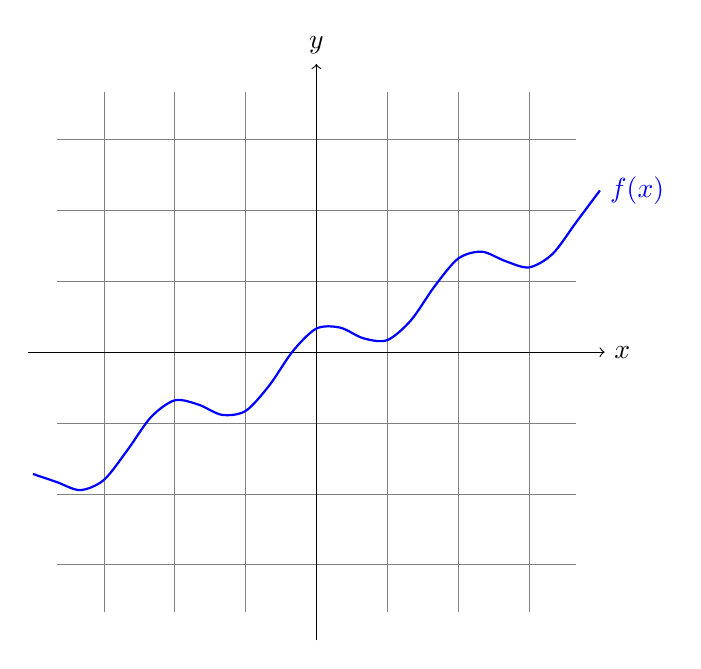
\begin{tikzpicture}[domain=-12:12, scale=0.3]
                \draw[very thin, step=3.0, color=gray] (-11, -11) grid (11, 11);
                \draw[->] (-12.2,0) -- (12.2,0) node[right] {$x$};
                \draw[->] (0,-12.2) -- (0,12.2) node[above] {$y$};
                \draw[smooth, thick, color=blue]   plot (\x,{cos(\x r) + \x / 2})   node[right] {$f(x)$};
            \end{tikzpicture}
        \end{center}

        \item Consider 
        \begin{align*}
            f: \realn &\longrightarrow \realn \\
            x &\longmapsto \begin{cases}
                1, & x \text{ rational} \\
                0, & x \text{ irrational}
            \end{cases}
        \end{align*}
        \begin{itemize}
            \item $x_0$ rational is a global maximum
            \item $x_0$ irrational is a global minimum
        \end{itemize}
    \end{enumerate}
\end{eg}

\begin{thm}
    Let $I$ be an open interval, and $f: I \realn \realn$ a function with a local extremum at $x_0 \in I$. Then
    \[
        f \text{ differentiable in } x_0 \implies f'(x_0) = 0
    \]
\end{thm}
\begin{proof}
    Assume $f'(x_0) \ne 0$ (w.l.o.g. $f'(x_0) > 0$, otherwise consider $-f$). Then 
    \begin{equation}
        \exists \delta > 0: ~~\left| \frac{f(x_0 + h) - f(x)}{h} - f'(x_0) \right| < f'(x_0) ~~\forall h \in (-\delta, \delta)
    \end{equation}
    Especially 
    \begin{equation}
        0 < \frac{f(x_0 + h) - f(x_0)}{h} ~~\forall h \in (-\delta, \delta)
    \end{equation}
    For $h > 0$ this means $f(x_0 + h) > f(x_0)$. And for $h < 0$ this means that $f(x_0 + h) < f(x_0)$. Thus $x_0$ is not an extremum.
\end{proof}

\begin{rem}
    Let $f: I \rightarrow \realn$ be differentiable. To find the extrema of $f$, calculate $f'$ and find its roots. 
    However, the roots are to be insepcted more closely, as $f'(x_0) = 0$ is not a sufficient criterion (The function could have inflection points or behave badly at the boundaries of $I$).
\end{rem}

\begin{thm}[Mean value theorem]
    Let $a, b \in \realn$ with $a < b$, and let $f, g: [a, b] \rightarrow \realn$ be differentiable. Then $\exists \xi \in (a, b)$ such that 
    \[
        (f(b) - f(a))g'(\xi) = f'(\xi)(g(b) - g(a))
    \]

    \begin{center}
        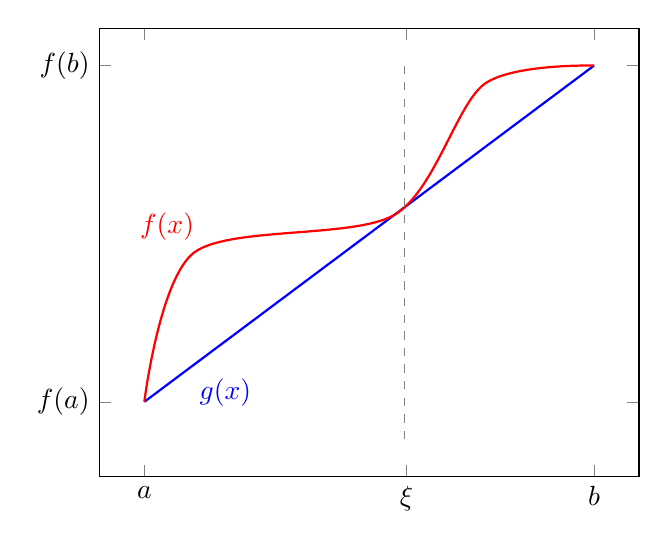
\begin{tikzpicture}
            \begin{axis}[ytick={1, 10}, yticklabels={$f(a)$, $f(b)$}, xtick={1, 6.25, 10}, xticklabels={$a$,$\xi$,$b$}]
                \addplot[thick, smooth, color=blue] coordinates {
                    (1, 1)
                    (10, 10)
                } node[below right, pos=0.1] {$g(x)$};

                \addplot[thick, smooth, color=red] coordinates {
                    (1, 1)
                    (2, 5)
                    (6, 6)
                    (7.8, 9.5)
                    (10, 10)
                }node[above left, pos=0.3] {$f(x)$};

                \addplot +[mark=none, dashed, gray] coordinates {(6.2, 0) (6.2, 10)};
            \end{axis}
        \end{tikzpicture}
    \end{center}
\end{thm}
\begin{proof}
    Consider all
    \begin{equation}
        h(x) = (f(b) - f(a))g(x) - f(x)(g(b) - f(a))
    \end{equation}
    $h$ is differentiable, which means $h$ is continuous on $[a, b]$:
    \begin{equation}
        h(a) = f(b)g(a) - f(a)g(b) = h(b)
    \end{equation}
    We need to show that $h'$ has a root in $[a, b]$. If $h$ is constant, this is trivial. So we assume $\exists x \in (a, b)$ such that $h(x) > h(a)$.
    Since $h$ is continuous on $(a, b)$ there exists a global maximum $x_0 \in [a, b]$ with $x_0 \ne a$ and $x_0 \ne b$. 
    This implies that $h'(x_0) = 0$. If $h(x) < h(a)$ the same argument can be made.
\end{proof}

\begin{rem}
    This theorem is often written as
    \[
        \frac{f(b) - f(a)}{g(b) - g(a)} = \frac{f'(\xi)}{g'(\xi)}
    \]
    And if $g(x) = x$
    \[
        \frac{f(b) - f(a)}{b - a} = f'(\xi)
    \]
\end{rem}

\begin{cor}
    Let $I$ be an open interval and $f: I \rightarrow \realn$ differentiable. Then 
    \begin{enumerate}[(i)]
        \item $f'(I) \subset [0, \infty) \iff \text{ monotonically increasing}$
        \item $f'(I) \subset (0, \infty) \implies \text{ strictly monotonically increasing}$
        \item $f'(I) \subset (-\infty, 0] \iff \text{ monotonically decreasing}$
        \item $f'(I) \subset (-\infty, 0) \implies \text{ striuctly monotonically decreasing}$
    \end{enumerate}
\end{cor}
\begin{proof}
    We will only show the "$\implies$" direction for (i). Assume $f$ isn't monotonically increasing, then $\exists x, y \in I$ such that $x < y$ but $f(x) > f(y)$.
    The mean value theorem thus states, $\exists \xi \in (x, y)$ such that
    \begin{equation}
        f'(\xi) = \frac{f(y) - f(x)}{y- x} < 0
    \end{equation}
    All other statements are proven in the same fashion.
\end{proof}

\begin{eg}
    $f$ strictly monotonically increasing does NOT imply that $f'(I) \subset (0, \infty)$. Consider $f(x) = x^3$.
\end{eg}

\begin{cor}[L'Hôpital's rule]
    Let $a, b, x_0 \in \realn$, with $a < x_0 < b$ and let $f, g: (a, b) \rightarrow \realn$ be a differentiable function. We require $f(x_0) = g(x_0) = 0$.
    If $g'(x) \ne 0 ~~\forall x \in I \setminus \set{x_0}$ and if 
    \[
        \limes{x}{x_0} \frac{f'(x)}{g'(x)}
    \]
    exists, then 
    \[
        \limes{x}{x_0} \frac{f(x)}{g(x)} = \limes{x}{x_0}\frac{f'(x)}{g'(x)}
    \]
\end{cor}
\begin{proof}
    Between two roots of $g$ there must be at least one root of $g'$. I.e. $g(x) \ne 0 ~~\forall x \in I \setminus \set{x_0}$.
    This means, that
    \begin{equation}
        \forall x \in (a, x_0) ~\exists \xi_x: ~~\frac{f(x)}{g(x)} = \frac{f(x) - f(x_0)}{g(x) - g(x_0)} = \frac{f'(\xi_x)}{g'(\xi_x)} \implies \limes{x}{x_0}\frac{f'(x)}{g'(x)}
    \end{equation}
    Since $\xi_x \in (x, x_0)$
    \begin{equation}
        \xi_x \conv{x \rightarrow x_0} x_0
    \end{equation}
    For the limit from the left, this implies 
    \begin{equation}
        \limes{x}{x_0} \frac{f(x)}{g(x)} = \limes{x}{x_0}\frac{f'(x)}{g'(x)}
    \end{equation}
    This argument can be made for the limit from the right as well.
\end{proof}

\begin{rem}
    \begin{enumerate}[(i)]
        \item For the computation of the limit it is enough to consider $f$ and $g$ on $(x_0 - \delta, x_0 + \delta)$ with $\delta > 0$.
        \item L'Hôpital's rule also works for one-sided limits
        \item Let $f, g: (a, b) \setminus \set{x_0} \rightarrow \realn$ be differentiable. Then it is enough to require 
        \[
            \limes{x}{x_0} f(x) = \limes{x}{x_0} g(x) = 0
        \]
        \item L'Hôpital's rule doesn't generally apply to complex valued functions.
        \item By substituring $\tilde{f}(x) = f\left(\frac{1}{x}\right)$ and $\tilde{g}(x) = g\left(\frac{1}{x}\right)$ we can also use 
        \[
            \limes{x}{\infty} \frac{\tilde{f}(x)}{\tilde{g}(x)} = \limes{x}{\infty} \frac{\tilde{f}'(x)}{\tilde{g}'(x)}
        \]
        \item The inverse 
        \[
            L = \limes{x}{x_0} \frac{f(x)}{g(x)} \implies \limes{x}{0} \frac{f'(x)}{g'(x)} = L
        \]
        is NOT true.
    \end{enumerate}
\end{rem}

\begin{eg}
    Consider 
    \[
        \limes{x}{0} \frac{x^2}{1 - \cos x} = \mathquotes{\frac{0}{0}}
    \]
    The functions here are 
    \begin{align*}
        f(x) = x^2 && g(x) = 1 - \cos x
    \end{align*}
    with the derivatives
    \begin{align*}
        f'(x) = 2x && g'(x) = \sin x
    \end{align*}
    However, the limit of the derivatives is still
    \[
        \limes{x}{0} \frac{2x}{\sin x} = \mathquotes{\frac{0}{0}}
    \]
    We can derive the functions again
    \begin{align*}
        f''(x) = 2 && g''(x) = \cos x
    \end{align*}
    And thus 
    \[
        \limes{x}{0} \frac{2}{\cos x} = 2 \implies \limes{x}{0} \frac{x^2}{1 - \cos x} = 2
    \]
\end{eg}

\begin{thm}[Derivative of inverse functions]
    Let $I$ be an open inverval, and $f: I \rightarrow \realn$ differentiable with $f'(I) \subset (0, \infty)$.
    Then $f$ has a differentiable inverse function $\inv{f}(x): f(I) \rightarrow \realn$ and for $y \in f(I)$ we have 
    \[
        \left(\inv{f}\right)'(y) = \frac{1}{f'\left(\inv{f}(y)\right)}
    \]
\end{thm}
\begin{proof}
    $f$ is strictly monotonically increasing, thus $\inv{f}$ exists and is continuous. Let $y \in f(I), ~x := \inv{f}(y)$ and 
    \begin{equation}
        \xi(h) = \inv{f}(y + h) - \underbrace{\inv{f}(y)}_x
    \end{equation}
    Then 
    \begin{equation}
        x + \xi(h) = \inv{f}(y + h) \implies f(x + \xi(h)) = y + h = f(x) + h
    \end{equation}
    Which in turn implies 
    \begin{equation}
        f(x + \xi(h)) - f(x) = h
    \end{equation}
    Now we have 
    \begin{equation}
    \begin{split}
        \frac{\inv{f}(y + h) - \inv{f}(y)}{h} =& \frac{\xi(h)}{f(x + \xi(h)) - f(x)} \\
        =& \inv{\left( \frac{f(x + \xi(h)) - f(x)}{\xi(h)} \right)} \\
        \conv{h \rightarrow 0}& \inv{\left(f'(x)\right)} = \frac{1}{f'(\inv{f}(y))}> 0
    \end{split}
    \end{equation}
\end{proof}

\begin{eg}
    \begin{enumerate}[(i)]
        \item Let $n \in \natn$ and consider 
        \begin{align*}
            f: (0, \infty) &\longrightarrow \realn \\
            x &\longmapsto x^n
        \end{align*}
        The derivative is $f'(x) = nx^{n-1}$. The inverse function is 
        \begin{align*}
            g(y) = \sqrt[n]{y} && g'(y) = \frac{1}{f'(g(y))} = \frac{1}{n\left(\sqrt[n]{y}\right)^{n-1}} = \frac{1}{n} \cdot y^{\left(\frac{1}{n} - 1\right)}
        \end{align*}

        \item The natural logarithm. Let $f(x) 0 \exp x$ and $g(y) = \ln y$. Then 
        \[
            (\ln y)' = \frac{1}{\exp(\ln(y))} = \frac{1}{y}
        \]

        \item Let $f(x) = x^3$. Then 
        \[
            \inv{f}(y) = \begin{cases}
                \sqrt[3]{y}, & y \ge 0 \\
                -\sqrt[3]{y}, & y < 0
            \end{cases}
        \]
        $\inv{f}$ is not differentiable in $y = 0$.
    \end{enumerate}
\end{eg}

\begin{defi}
    Let $I$ be an open interval. $f: I \rightarrow \realn$ is said to be $(n+1)$-times differentiable if the $n$-th derivative of $f$ ($f^{(n)}$) is differentiable.
    
    $f$ is said to be infinitely differentiable (or smooth) if $f$ is $n$ times differentiable for all $n \in \natn$.

    $f$ is said to be $n$ times continuously differentiable if the $n$-th derivative $f^{(n)}$ is continuous.
\end{defi}

\begin{defi}
    Let $I$ be an open interval, and $f: I \rightarrow \realn$ $n$ times differentiable in $x \in I$. Then 
    \[
        T_n f(y) = \sum_{k=0}^n \frac{f^{(k)} (x)}{k!} (y - x)^k
    \]
    is called the Taylor polynomial of $n$-th degree at $x$ of $f$.
\end{defi}

\begin{thm}[Taylor's theorem]
    Let $I$ be an open interval and $f: I \rightarrow \realn$ an $(n+1)$-times differentiable function.
    Let $x \in I$ and $h: I \rightarrow \realn$ differentiable. For every $y \in I$, there exists a $\xi$ between $x$ and $y$ such that 
    \[
        (f(y) - T_n f(y)) \cdot h'(\xi) = \frac{f^{(n+1)}(\xi)}{n!} (y - \xi)^n (h(y) - h(x))
    \]
\end{thm}
\begin{proof}
    Let 
    \begin{equation}
    \begin{split}
        g: I &\longrightarrow \realn \\
        t &\longmapsto \sum_{k=0}^n \frac{f^{(k)}(t)}{k!} (y-t)^k
    \end{split}
    \end{equation}
    Apply the mean value theorem to $g$ and $h$ to  get 
    \begin{equation}
        g'(\xi)(h(y) - h(x)) = (g(y) - g(x))h'(\xi) = (f(y) - T_nf(y))h'(\xi)
    \end{equation}
    and thus 
    \begin{equation}
    \begin{split}
        g'(t) &= \sum_{k=0}^n \underbrace{\left( \frac{f^{(k+1)}(t)}{k!} (y-t)^k - \frac{f^{(k)}(t)}{k!}k(y - t)^{k-1} \right)}_{\text{Telescoping series}} \\
        &= \frac{f^{n+1}(t)}{n!} (y-t)^n
    \end{split}
    \end{equation}
    By inserting $\xi$ we receive the desired equation.
\end{proof}

\begin{rem}
    \begin{enumerate}[(i)]
        \item This is useful for when $h'(\xi) \ne 0$
        \item The choice of $h$ can yield different errors
        \[
            R_{n+1}(y, x) := f(y) - T_nf(y)
        \]
        \item The Langrange error bound is for $h(t) = (y - t)^{n+1}$:
        \[
            R_{n+1}(y, x) = \frac{f^{(n+1)}(\xi)}{(n+1)!} (y-x)^{n+1}
        \]
        \item This theorem makes no statement about Taylor series.
    \end{enumerate}
\end{rem}

\begin{cor}
    Let $(a, b) \subset \realn$ and $f: (a, b) \rightarrow \realn$ a $n$-times continuously differentuable function with 
    \[
        0 = f'(x) = f''(x) = \cdots = f^{(n-1)}(x)
    \]
    and $f^{(n)} \ne 0$. If $n$ is odd, then there is no local extremum in $x$. If $n$ is even then 
    \begin{align*}
        f^{(n)}(x) > 0 &\implies x \text{ is a local maximum} \\
        f^{(n)}(x) < 0 &\implies x \text{ is a local minimum}
    \end{align*}
\end{cor}
\begin{proof}
    W.l.o.g. $f^{(n)} > 0$. We will use the Taylor series with Lagrange error bound. 
    According to prerequisites, $f^{(n)}$ is continuous, i.e. $\exists \epsilon > 0$ such that $f^{(n)}(\xi) > 0$ on $(x - \epsilon, x + \epsilon)$.
    The Taylor formula tells us, that $\forall y \in (x - \epsilon, x + \epsilon) ~\exists \xi_y \in (x - \epsilon, x + \epsilon)$ such that
    \begin{equation}
        f(y) - T_{n-1}(f(y)) = f(y) - f(x) = \frac{f^{(n)}(\xi_y)}{n!} (y - x)^n
    \end{equation}
    For $n$ odd, $f(y) - f(x)$ assumes positive and negative values in every neighbourhood of $x$. If $n$ is even then $f(y) - f(x)$ cannot be negative, thus $x$ is a local minimum.
\end{proof}
\end{document}